% Copyright 2004 by Till Tantau <tantau@users.sourceforge.net>.
%
% In principle, this file can be redistributed and/or modified under
% the terms of the GNU Public License, version 2.
%
% However, this file is supposed to be a template to be modified
% for your own needs. For this reason, if you use this file as a
% template and not specifically distribute it as part of a another
% package/program, I grant the extra permission to freely copy and
% modify this file as you see fit and even to delete this copyright
% notice. 

\documentclass{beamer}

% There are many different themes available for Beamer. A comprehensive
% list with examples is given here:
% http://deic.uab.es/~iblanes/beamer_gallery/index_by_theme.html
% You can uncomment the themes below if you would like to use a different
% one:
%\usetheme{AnnArbor}
%\usetheme{Antibes}
%\usetheme{Bergen}
%\usetheme{Berkeley}
%\usetheme{Berlin}
%\usetheme{Boadilla}
%\usetheme{boxes}
%\usetheme{CambridgeUS}
%\usetheme{Copenhagen}
%\usetheme{Darmstadt}
\usetheme{default}
%\usetheme{Frankfurt}
%\usetheme{Goettingen}
%\usetheme{Hannover}
%\usetheme{Ilmenau}
%\usetheme{JuanLesPins}
%\usetheme{Luebeck}
%\usetheme{Madrid}
%\usetheme{Malmoe}
%\usetheme{Marburg}
%\usetheme{Montpellier}
%\usetheme{PaloAlto}
%\usetheme{Pittsburgh}
%\usetheme{Rochester}
%\usetheme{Singapore}
%\usetheme{Szeged}
%\usetheme{Warsaw}

\usepackage{setspace} 
\usepackage{amsmath}
\usepackage{graphicx}
\newcommand*{\LargerCdot}{\raisebox{-0.25ex}{\scalebox{2.3}{$\cdot$}}}

\usepackage{color}
%\input{rgb}

\definecolor{red1}{rgb}{1.000000,0.000000,0.000000}

\title{Signal Processing Challenge}

% A subtitle is optional and this may be deleted
%\subtitle{A study of Turbulence in Financial Markets}

\author{Ranaji~Krishna}
% - Give the names in the same order as the appear in the paper.
% - Use the \inst{?} command only if the authors have different
%   affiliation.

%\institute[Universities of Somewhere and Elsewhere] % (optional, but mostly needed)
%{
%  \inst{1}%
%  Summer Intern\\
%  Research Affiliates
%  \and
%  \inst{2}%
%  Vice President Research\\
%  Research Affiliates}
% - Use the \inst command only if there are several affiliations.
% - Keep it simple, no one is interested in your street address.

%\date{2013}
% - Either use conference name or its abbreviation.
% - Not really informative to the audience, more for people (including
%   yourself) who are reading the slides online

\subject{Theoretical Computer Science}
% This is only inserted into the PDF information catalog. Can be left
% out. 

% If you have a file called "university-logo-filename.xxx", where xxx
% is a graphic format that can be processed by latex or pdflatex,
% resp., then you can add a logo as follows:

\pgfdeclareimage[height=0.6cm]{university-logo}{sys_logo.jpeg}
\logo{\pgfuseimage{university-logo}}

% Delete this, if you do not want the table of contents to pop up at
% the beginning of each subsection:
%\AtBeginSubsection[]
%{
%  \begin{frame}<beamer>{Outline}
%    \tableofcontents[currentsection,currentsubsection]
%  \end{frame}
%}^6

% Let's get started
\begin{document}

\begin{frame}
  \titlepage
\end{frame}

%\begin{frame}{Outline}
%%	\begin{scriptsize}
%	 		\tableofcontents
%%  		% You might wish to add the option [pausesections]
%%	\end{scriptsize}
%\end{frame}

% Section and subsections will appear in the presentation overview
% and table of contents.
%\section{\small{Turbulence}}
	%\section{\small{The Concept of Financial Turbulence}}
	%\section{Turbulence as a measure of Systemic risk}
	% What are the other forms of systemic risk

%\setlength\listparindent{1in}

\begin{frame}{Problem Statement}{}
	\begin{itemize}
		\item{Assume a data matrix X with the following model:} \vspace{0 in}
		\begin{equation}
			X = A_{s} B^{T}_{s} + A_{n} B^{T}_{n}+ Z
		\end{equation}  where \newline
		{$\LargerCdot$ $X$ is a real ($m \times n$) matrix;}\newline 
		{$\LargerCdot$ $A_{n}$ is an unknown ($m \times d$) matrix, where the exact value of $d$ is not known, but $d << m,n$;}\newline 
		{$\LargerCdot$ $B_n$ is an unknown ($n \times d$) matrix;}\newline 
		{$\LargerCdot$ $A_s$ is an unknown ($m \times q$) matrix, where $q$ is known, and $q << m,n$. Also each column of $A_s$ is in the column span of a \textit{known} matrix $S$;}\newline 
		{$\LargerCdot$ $B_s$ is an unknown ($n \times q$) matrix. But each row of $B_s$ has at most one non-zero element.}\newline 
		{$\LargerCdot$ It is assumed that span($A_n$)  $\not\subset$ span($A_s$).}\newline 
		\item{Find a computation efficient method to estimate $A_s$ and $B_s$.} \vspace{0.5 in}
	\end{itemize}
\end{frame}


\begin{frame}{Approach}{}
	\begin{itemize}	
		\item{Use the technique of {\color{blue}Singular Value Decomposition} to estimate $A_s$ and $B_s$. } \newline	
		\item{Matrix $X$ can be expressed as:}
		\begin{equation}
			X = U \Sigma V^T
		\end{equation}  where \newline
		{$\LargerCdot$ $U$ is a real ($m \times m$) matrix of eigenvectors of $XX^T$ ;}\newline 
		{$\LargerCdot$ $\Sigma$ is a real ($m \times m$) diagonal matrix of eigenvalues of $XX^T$;}\newline 
		{$\LargerCdot$ $V$ is a real ($n \times m$) matrix of eigenvectors of $X^TX$ that correspond to non-zero eigenvalues.}\newline 
		\item{Setting $A_s$ = $U\Sigma$, places $A_s$ in the column span of matrix $U$, a \textit{known} matrix. This implies $B_s$ = $V$. When the eigenvectors of the highest $q$ eigenvalues are selected, $U$ is an ($m \times q$), $\Sigma$ is a ($q \times q$) and $V$ is a ($n \times q$) matrix.} \vspace{0.2 in}
	\end{itemize}
\end{frame}


\begin{frame}{Simulation Framework}{}
	\begin{itemize}
		\item{The performance was tested for the following simulation parameters:}\vspace{0.1 in}\newline
		{$\LargerCdot$ Entries of $A_s$ are derived from the class of random staircase functions, of integer 					step heights and width 32.\newline In the Matlab notation:
					kron(randi(8, m/32, 1), ones(32, 1)),  and in R notation: kronecker(runif(m/32, 1, 8), rep(1, 32))}\newline
		{$\LargerCdot$ Rows of $B_s$ are zero except for possibly one random location where it is one.}\newline
		{$\LargerCdot$ Entries of $B_n$ are i.i.d samples from a Gaussian process of a given variance.}\newline
		{$\LargerCdot$ Columns of $A_n$ are random traces of a random walk process.}\newline
		{$\LargerCdot$ $m=256,q=4,d=16,n=1024$.}
	\end{itemize}
\end{frame}


\begin{frame}{Results}{}
	\begin{itemize}		
		\item{LHS: Plot of Signal (typical column of matrix $X$); \newline
		RHS: Actual and Estimated values of $A_sB^T_s$ for the Signal.}\vspace{0 in}				
	\begin{figure}
		\begin{itemize}
			\begin{center}
				\vspace*{-0.1 in}
				\hspace*{-0.6in}
				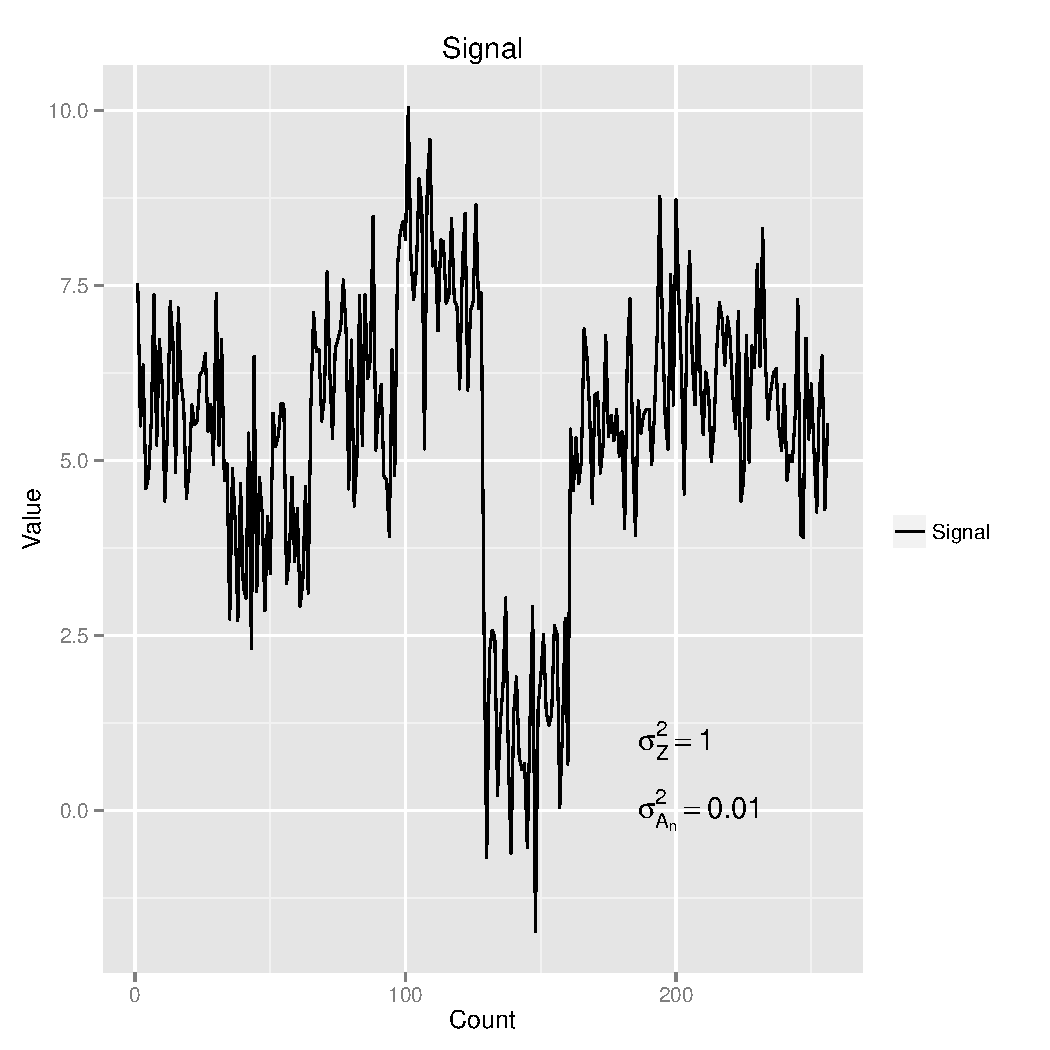
\includegraphics[width=0.55\textwidth]{Signal.pdf} 
	 			 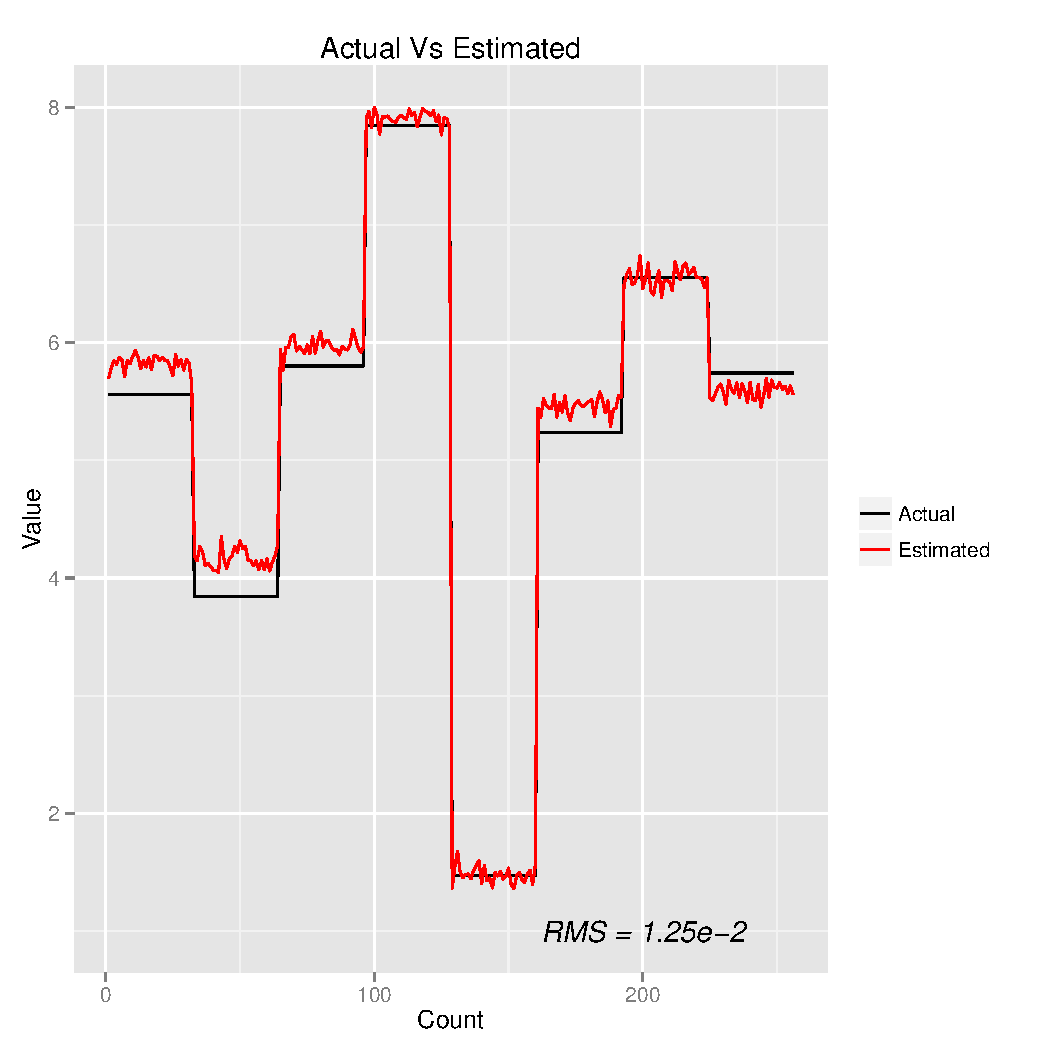
\includegraphics[width=0.55\textwidth]{SVDperf.pdf} 
			\end{center}
		\end{itemize}
	\end{figure}
		\vspace{-0.in}
		\end{itemize}
\end{frame}


\begin{frame}{Results}{contd.}
	\begin{itemize}
		\vspace{-0 in}		
		\item{Similarity between the actual ($A_sB_s^T$) and estimated matrix ($\hat{A}_s\hat{B}_s^T$) is used as a performance measure. Similarity is evaluated using Root-Mean-Square}, \newline\vspace{0 in}
		\begin{equation}
			rms = \frac{1}{nm}\sqrt{\sum_{j=1}^{m}\sum_{i=1}^{n} \Big((A_sB_s^T)_{j, i} - (\hat{A}_s\hat{B}_s^T)_{j, i}\Big)^2}
		\end{equation} \newline
%	\begin{figure}
%		\begin{itemize}
%			\begin{center}
%				\vspace*{-0.5 in}
%				\hspace*{-0.7in}
%				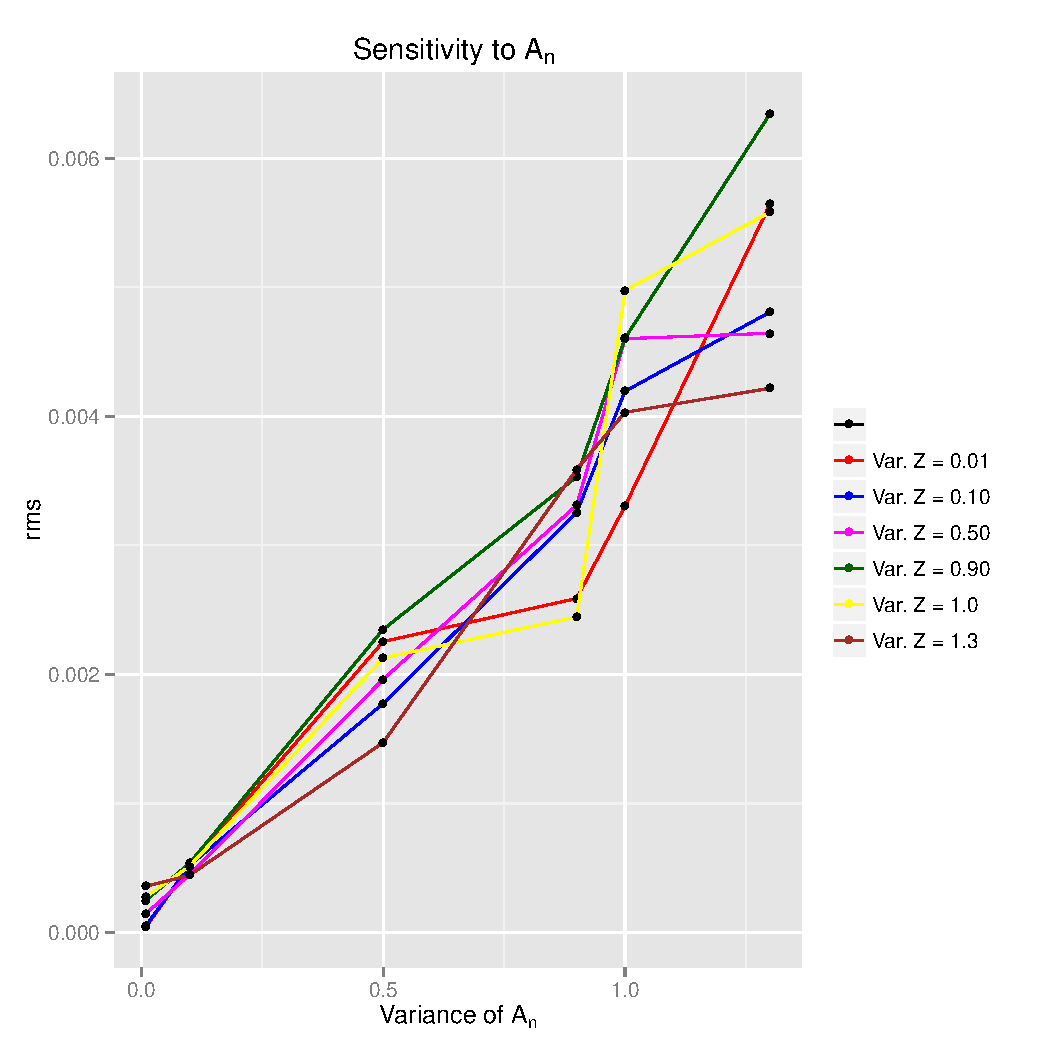
\includegraphics[width=0.55\textwidth]{SenA.pdf} 
%	 			 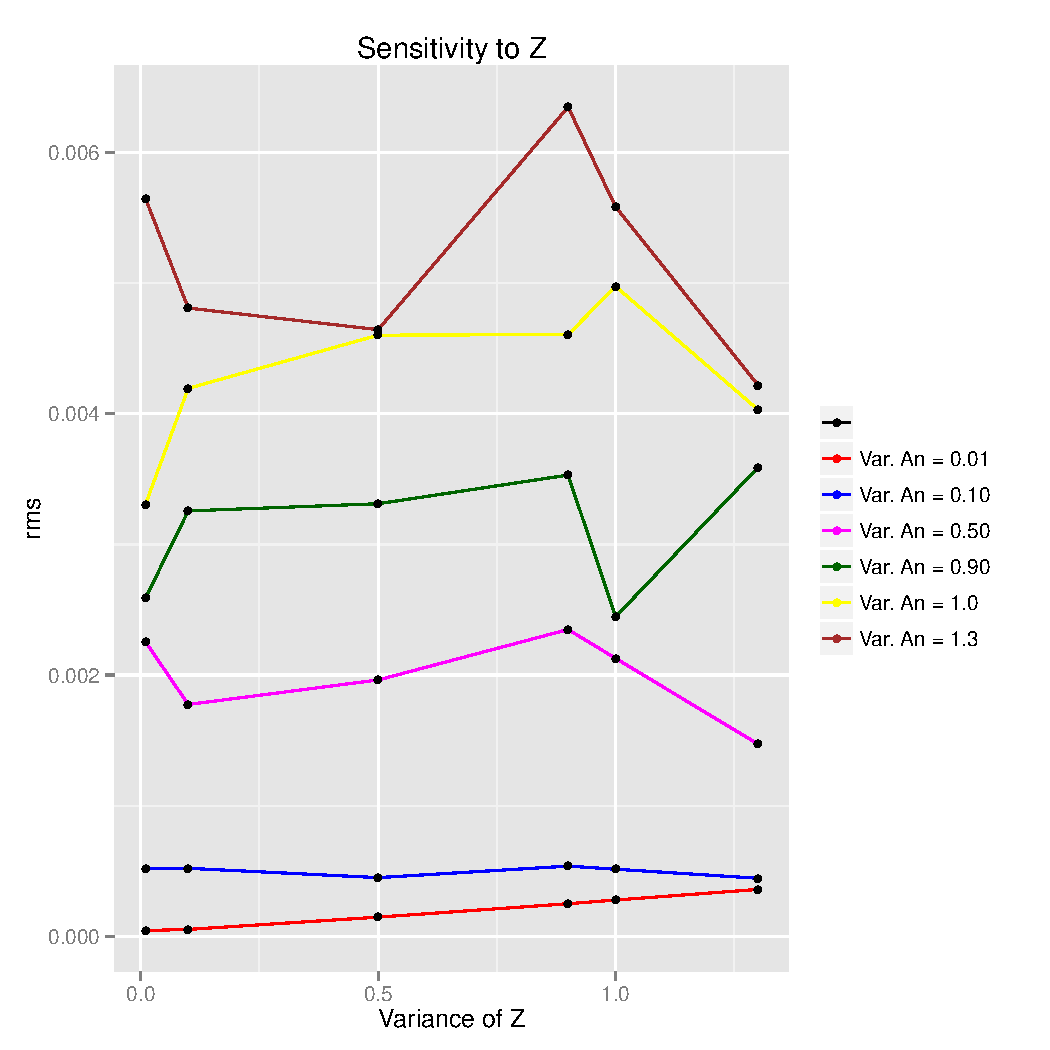
\includegraphics[width=0.55\textwidth]{SenZ.pdf} 
%			\end{center}
%		\end{itemize}
%	\end{figure}
		\vspace{-0.in}
		\end{itemize}
\end{frame}


\begin{frame}{Results}{contd.}
	\begin{figure}
	\vspace{-0.3 in}
		\begin{itemize}\item{Sensitivity to variance in $A_n$ and in $Z$}, \newline\vspace{-0 in}
			\begin{center}
				\vspace*{-0.1 in}
				\hspace*{-0.4in}
				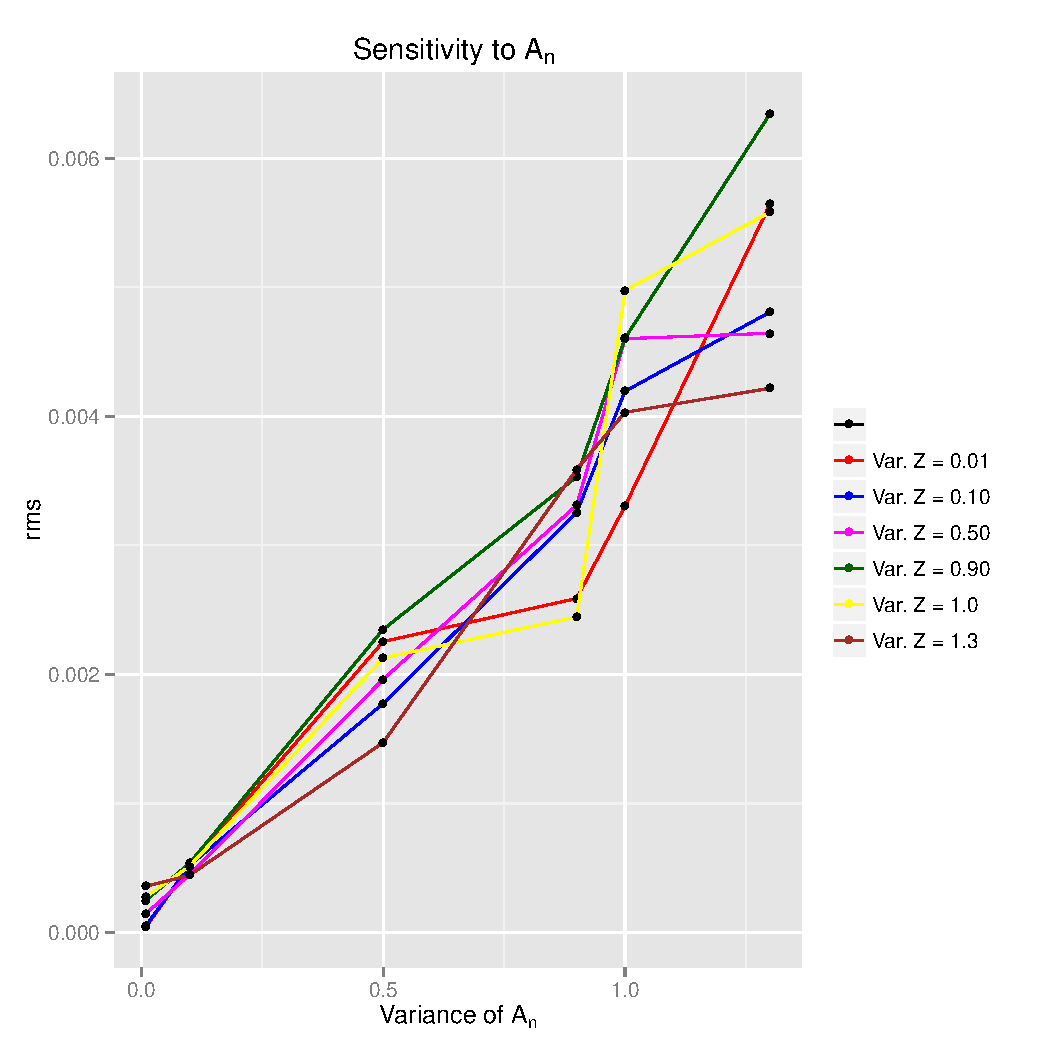
\includegraphics[width=0.55\textwidth]{SenA.pdf} 
	 			 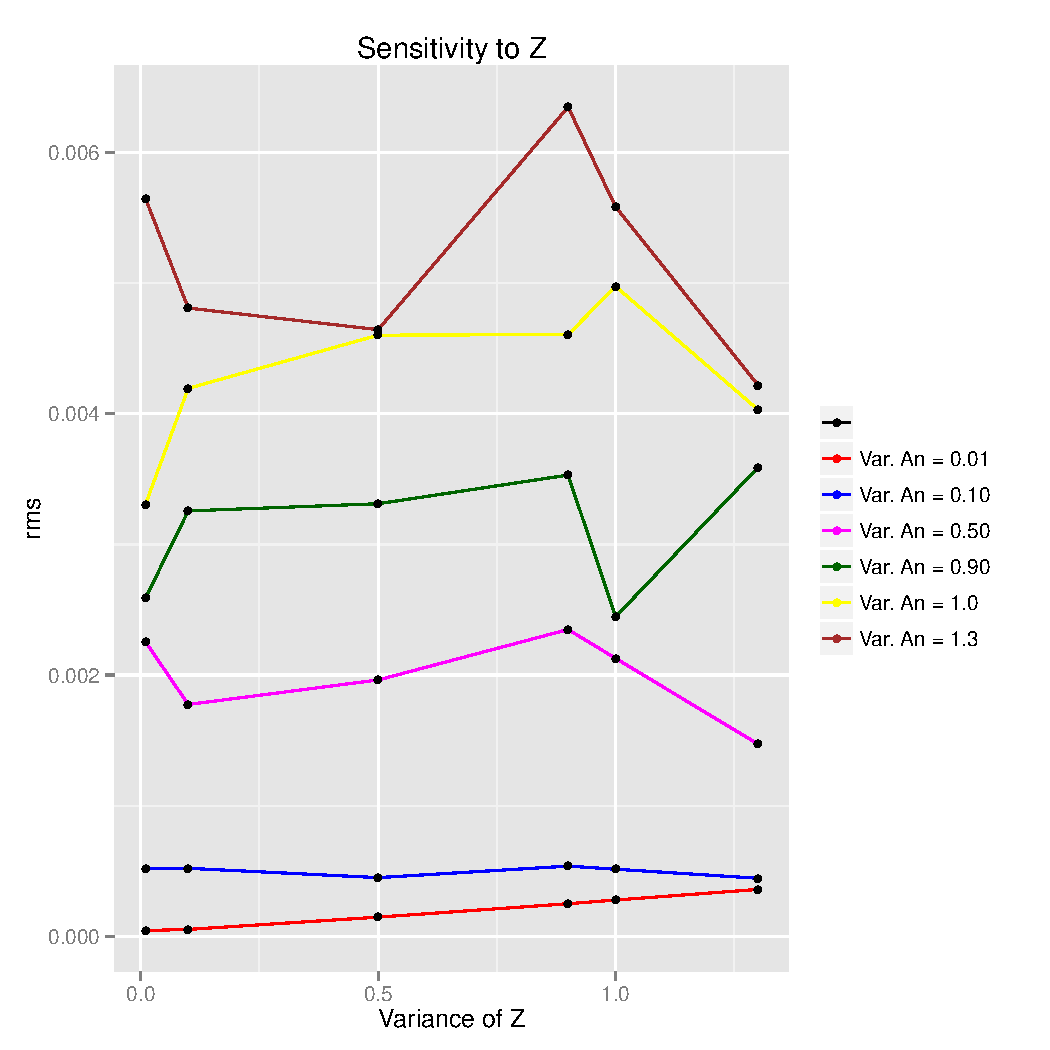
\includegraphics[width=0.55\textwidth]{SenZ.pdf} 
			\end{center}
		\end{itemize}
	\end{figure}
		\vspace{-0.in}
\end{frame}

\begin{frame}{Results}{contd.}
	\begin{figure}
	\vspace{-0.3 in}
		\begin{itemize}\item{Sensitivity to variance in $q$ and in $d$}, \newline\vspace{-0 in}
			\begin{center}
				\vspace*{-0.1 in}
				\hspace*{-0.4in}
				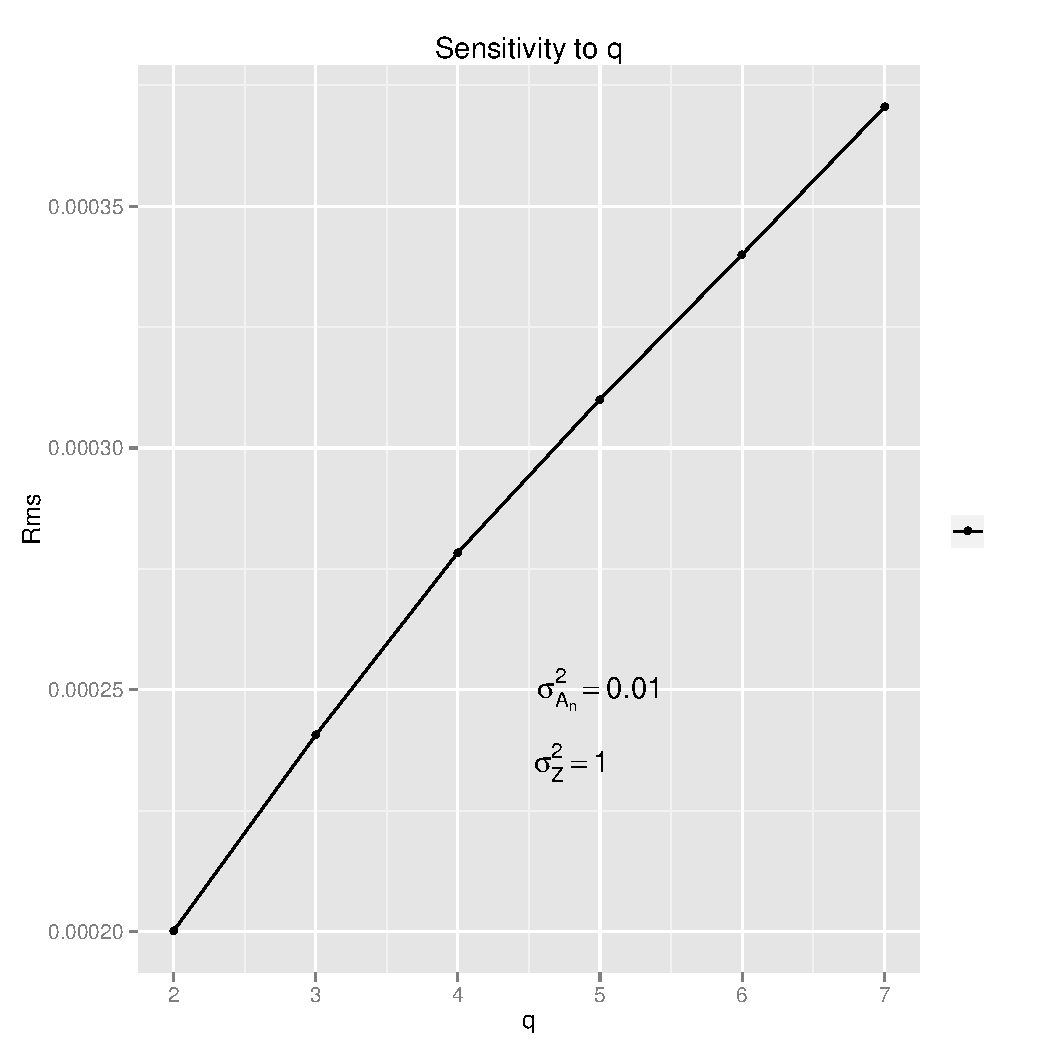
\includegraphics[width=0.55\textwidth]{Sen_q.pdf} 
	 			 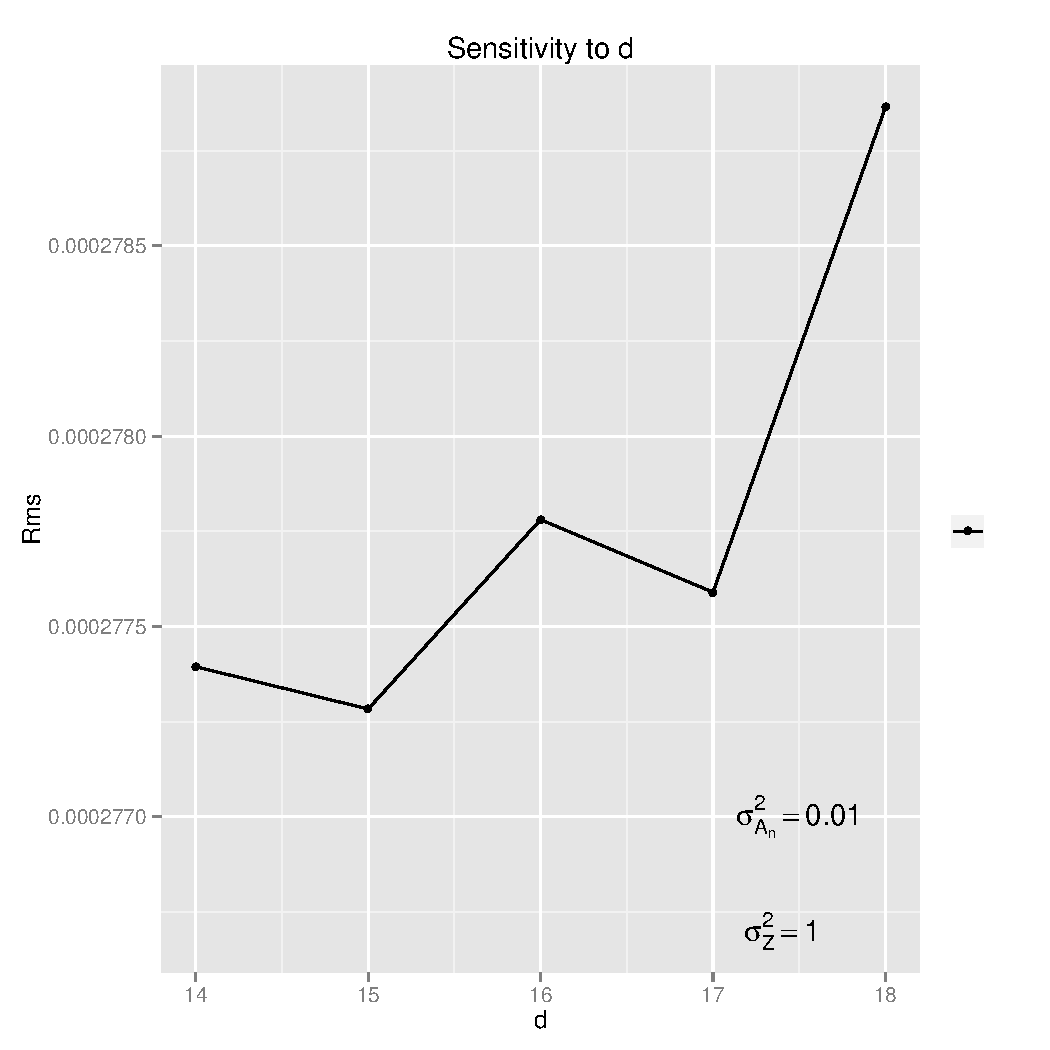
\includegraphics[width=0.55\textwidth]{Sen_d.pdf} 
			\end{center}
		\end{itemize}
	\end{figure}
		\vspace{-0.in}
\end{frame}

\begin{frame}{}{}
	\begin{center}
        		\Large{END}          
      \end{center}
\end{frame}


% All of the following is optional and typically not needed. 
%\appendix
%\section<presentation>*{\appendixname}
%\subsection<presentation>*{For Further Reading}
%
%\begin{frame}[allowframebreaks]
%  \frametitle<presentation>{For Further Reading}
%    
%  \begin{thebibliography}{10}
%    
%  \beamertemplatebookbibitems
%  % Start with overview books.
%
%  \bibitem{Author1990}
%    A.~Author.
%    \newblock {\em Handbook of Everything}.
%    \newblock Some Press, 1990.
% 
%    
%  \beamertemplatearticlebibitems
%  % Followed by interesting articles. Keep the list short. 
%
%  \bibitem{Someone2000}
%    S.~Someone.
%    \newblock On this and that.
%    \newblock {\em Journal of This and That}, 2(1):50--100,
%    2000.
%  \end{thebibliography}
%\end{frame}

\end{document}
